\DiaryEntry{Differential Coding}{2021-08-11}{Coding}

Correlation between samples imposes a structure on the data which can be exploited for compression in a number of different ways. In vector quantization, we used the fact that if we partition a correlated sequence into vectors, these vectors will cluster or aggregate in a very small part of the available space. By focusing our resources on accurately covering this restricted space, or vector quantization, we were able to obtain efficient compression.

Here, we look at a very different way of making use of the structure gifted to us by the correlation between samples. Because neighboring samples are correlated, we can predict the value of the sample we are trying to encode based on the values of past samples with some degree of accuracy. The difference between the actual and predicted values should then, on the average, have a smaller dynamic range than the dynamic range of the values of the original sample. In a sense, we are again clustering or aggregating the values that need to be represented, albeit in only one dimension. This allows us to use scalar quantizers in a more effective manner. The fact that we are encoding differences gives us the name differential encoding. Because the prediction techniques are rather simple, these schemes are much easier to implement than other compression schemes.

\subsection{Introduction}

We have a sequence of input values $\{x_n\}$ we want to quantize. Howeve,r we do not directly quantize the seuqnece, but consider the difference sequence $\{ d_n = x_n - x_{n-1} \}$ instead. In many sources of interest, the sampled source output {xn } does not change a great deal from one sample to the next. This means that both the dynamic range and the variance of the difference sequence $d_n$ are significantly smaller than that of the source output sequence. Furthermore, for correlated sources the distribution of dn is highly peaked at zero.

Given the relationship between the variance of the quantizer input and the incurred quantization error, it is also useful, in terms of lossy compression, to look at ways to encode the difference from one sample to the next rather than encoding the actual sample value. Techniques that transmit information by encoding differences are called \emph{differential encoding techniques}.

\paragraph{Example.} COnsider an input sequence $\{ x_n \}$ of

\bee
6.2, 9.7, 13.2, 5.9, 8, 7.4, 4.2, 1.8
\eee

The difference sequence $\{ d_n \}$ is given by (we are assuming that $x_{-1} = 0$),

\bee
6.2, 3.5, 3.5, -7.3, 2.1, -0.6, -3.2, -2.4
\eee

Suppose we use a quantizer with seven levels; decision boundaries are $-5, -3, -1, 1, 3, 5$ and corresponidng output values are $-6, -4, -2, 0, 2, 4, 6$. If we quantize the difference sequence $d_n$ with this quantizer, we obtain the following values $\Qc(d_n)$,

\bee
6, 4, 4, -6, 2, 0, -4, -2
\eee

Now we transmit the sequence and reconstruct the original sequence using the quantized difference. We obtain

\bee
6, 10, 14, 8, 10, 10, 6, 4
\eee

So far so good, but we see that the reconstruction gets worse with time. \qed

To better understand what's happening, let's write things down. We have the sequence $\{ x_n\}$ and obtain the difference sequence $\{d_n  = x_n - x_{n-1}\}$. Quantization yields the sequence $\{ \hat d_n \}$ with

\bee
\hat d_n = Q(d_n) = d_n + q_n
\eee

where $q_n$ is the quantization error. At the receiver, we obtain the reconstructed sequence $\{ \hat x_n \}$ as follows

\bee
\hat x_n = \hat x_{n-1} + \hat d_n
\eee

Let's play this through for the first two values.

\begin{align*}
  d_1 &= x_1 - x_0 \\
  \hat d_1 &= Q(d_1) = d_1 + q_1 \\
  \hat x_1 &= x_0 + \hat d_1 = x_0 + d_1 + q_1 = x_1 + q_1 \\
  d_2 &= x_2 - x_1 \\
  \hat d_2 &= Q(d_2) = d_2 + q_2 \\
  \hat x_2 &= \hat x_1 + \hat d_2 = x_1 + q_1 + d_2 + q_2 = x_2 + q_1 + q_2
\end{align*}
             
In general, we see that

\bee
\hat x_n = x_n + \sum_k q_k
\eee

We can see that the quantization error accumulates as the process continues. Theoretically, if the quantization error process is zero mean, the errors will cancel each other out in the long run. In practice, often long before that can happen, a significant error will have built up.


The underlying problem is that the encoder and decoder are operating with different pieces of information. The encoder generates the difference sequence based on the original sample values, while the decoder adds back the quantized difference onto a distorted version of the original signal. We can solve this problem by having both encoder and decoder use the same information during the differencing and reconstruction operations. The only information available to the receiver about the sequence $\{ x_n\}$ is the reconstructed sequence $\{ \hat x_n\}$. As this information is also available to the transmitter, we can modify the differencing operation to use the reconstructed value of the previous sample, instead of the previous sample itself. So we have

\bee
d_n = x_n - \hat x_{n-1}
\eee

If we now play through the scenario of the first two values, we obtain

\begin{align*}
  d_1 &= x_1 - x_0 \\
  \hat d_1 &= Q(d_1) = d_1 + q_1 \\
  \hat x_1 &= x_0 + \hat d_1 = x_0 + d_1 + q_1 = x_1 + q_1 \\
  d_2 &= x_2 - \hat x_1 \\
  \hat d_2 &= Q(d_2) = d_2 + q_2 \\
  \hat x_2 &= \hat x_1 + \hat d_2 = \hat x_1 + d_2 + q_2 = x_2 + q_2
\end{align*}

And in general, we see that

\bee
\hat x_n = x_n + q_n
\eee

There is no more accumulation of the quantization noise. In fact, the quantization noise in the $n$-th reconstructed sequence is the quantization noise incurred by the quantization of the $n$-th difference. The quantization error for the difference sequence is substantially less than the quantization error for the original sequence. Therefore, this procedure leads to an overall reduction of the quantization error. If we are satisfied with the quantization error for a given number of bits per sample, then we can use fewer bits with a differential encoding procedure to attain the same distortion.

A block diagram of the encoder / decoder structure is shown in the following Figure.


\begin{figure}[H]
    \centering
    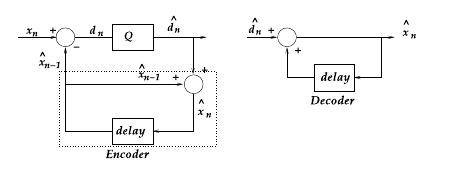
\includegraphics[scale=0.7]{images/2021-08-11-diff_enc_01.png}
\end{figure}

We would like our difference value to be as small as possible. For this to happen, given the system we have described to this point, $\hat x_n$ should be as close to $x_n$ as possible. However, $\hat x_-n$ is the reconstructed value of $x_n$; therefore, we would like $\hat x_n$ to be close to $x_n$. Unless $x_{n-1}$ is always very close to $x_n$ , some function of past values of the reconstructed sequence can often provide a better prediction of $x_n$. We therefore define a generic predictor function which provides a prediction for $x_n$ based on the past observed values,

\bee
p_n = f(\hat x_{n-1}, \hat x_{n-2}, \ldots)
\eee

For computational purposes, the predictor function can only take a finite number of past inputs. A corresponding block diagram of this more general structure is shown in the following Figure.

\begin{figure}[H]
    \centering
    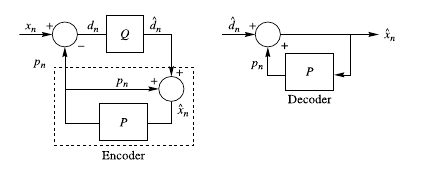
\includegraphics[scale=0.7]{images/2021-08-11-diff_enc_02.png}
\end{figure}

This basic differential encoding system is known as the differential pulse code modulation (DPCM) system.




%%% Local Variables:
%%% mode: latex
%%% TeX-master: "journal"
%%% End:
